\begin{figure}[htbp]\centering
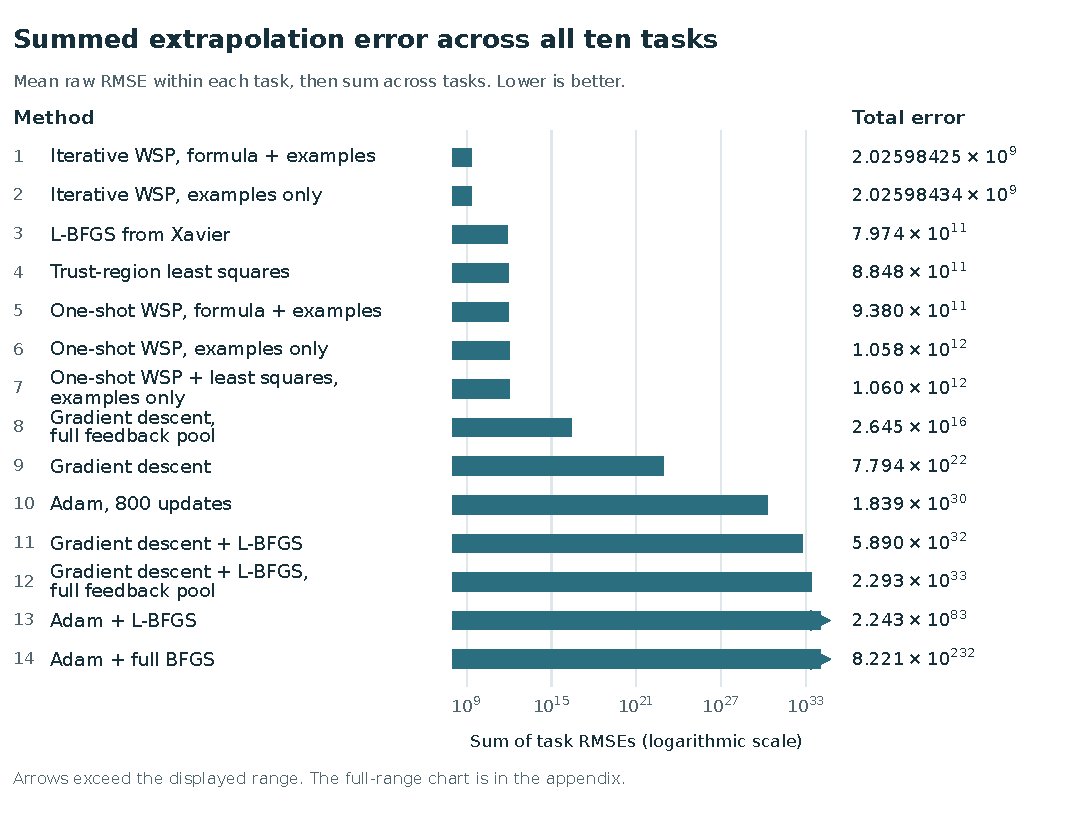
\includegraphics[width=\linewidth]{holistic_main.pdf}
\caption{\textbf{Iterative WSP has the lowest summed raw extrapolation error in this benchmark.} Each method is evaluated on the same 87 task, architecture and start combinations. For each task, we average raw root mean squared error (RMSE) across its tested sizes and three starts, then sum those ten task values. Each task contributes one mean; output scales are not normalized. Ranks use unrounded totals. The two iterative WSP totals agree to six significant figures. The full feedback-pool controls use additional labels, and WSP followed by least squares receives an additional numerical stage. Adam means adaptive moment estimation; BFGS means Broyden--Fletcher--Goldfarb--Shanno. Fibonacci supplies 99.8\% of the examples-only one-shot total; positive self-power supplies 78.1\% of its iterative counterpart. The horizontal axis is logarithmic. Arrows mark the two totals beyond $10^{34}$, with their actual values printed at the right. Figure~\ref{fig:holisticfull} shows the entire range.}\label{fig:holisticraw}
\end{figure}
